\usetikzlibrary{arrows.meta,calc}
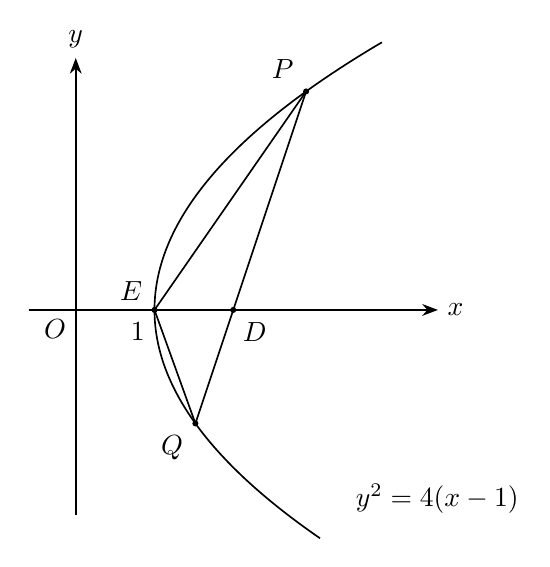
\begin{tikzpicture}[x=1cm,y=1cm,line width=.6pt,font=\normalsize]
\tikzset{ptlabel/.style={font=\normalsize,fill=none,inner sep=1.2pt}}
% Axes
\draw[-{Stealth[length=2mm]}] (0,-2.6) -- (0,3.2);
\draw[-{Stealth[length=2mm]}] (-0.6,0) -- (4.6,0);
\node[ptlabel,above,yshift=2pt] at (0,3.2) {$y$};
\node[ptlabel,right,xshift=2pt] at (4.6,0) {$x$};
\node[ptlabel,below left,xshift=-2pt,yshift=-2pt] at (0,0) {$O$};
% Parabola y^2=4(x-1), i.e. x=1+y^2/4, exact formula plot
\draw[domain=-2.9:3.4,samples=120,smooth,variable=\t] plot ({1+\t*\t/4},{\t});
\node[ptlabel,right=3pt] at (3.4,-2.4) {$y^{2}=4(x-1)$};
% Points: E vertex (1,0), D(2,0), P upper, Q lower on parabola, secant PQ through D
\coordinate (E) at (1,0);
\coordinate (D) at (2,0);
\coordinate (P) at (2.924950591,2.774851773);
\coordinate (Q) at (1.519493853,-1.44151844);
% triangle EPQ + secant PQ through near D (schematic, original not to scale)
\draw (E) -- (P);
\draw (E) -- (Q);
\draw (P) -- (Q);
\fill (E) circle (1.1pt);
\fill (D) circle (1.1pt);
\fill (P) circle (1.1pt);
\fill (Q) circle (1.1pt);
\node[ptlabel,above left,xshift=-3pt,yshift=2pt] at (E) {$E$};
\node[ptlabel,below left,xshift=-2pt,yshift=-3pt] at (1,0) {$1$};
\node[ptlabel,below right,xshift=2pt,yshift=-3pt] at (D) {$D$};
\node[ptlabel,above left,xshift=-3pt,yshift=3pt] at (P) {$P$};
\node[ptlabel,below left,xshift=-3pt,yshift=-3pt] at (Q) {$Q$};
\end{tikzpicture}
